% Created 2018-11-27 Tue 00:40
% Intended LaTeX compiler: pdflatex
\documentclass[11pt]{article}
\usepackage[utf8]{inputenc}
\usepackage[T1]{fontenc}
\usepackage{graphicx}
\usepackage{grffile}
\usepackage{longtable}
\usepackage{wrapfig}
\usepackage{rotating}
\usepackage[normalem]{ulem}
\usepackage{amsmath}
\usepackage{textcomp}
\usepackage{amssymb}
\usepackage{capt-of}
\usepackage{hyperref}
\date{\textit{[2018-11-26 Mon]}}
\title{BBB Testing Documentation}
\hypersetup{
 pdfauthor={},
 pdftitle={BBB Testing Documentation},
 pdfkeywords={},
 pdfsubject={},
 pdfcreator={Emacs 26.1 (Org mode 9.1.14)}, 
 pdflang={English}}
\begin{document}

\maketitle
\tableofcontents


\section{Iteration 1}
\label{sec:orga319995}

\subsection{Specify Test Cases}
\label{sec:org9433063}

\subsubsection{Class Ticket}
\label{sec:orgd6ffa7f}

\begin{description}
\item[{\textbf{TC\_Ticket\_1}}] initializes correctly
\begin{description}
\item[{Class}] Ticket
\item[{Method}] constructor
\item[{Precondition}] N/A
\item[{Input}] \{ id: “T1”, seat: 1 \}
\item[{Expected Output}] Ticket\{ id: “T1”, seat: 1, boarded: false \}
\end{description}

\item[{\textbf{TC\_Ticket\_2}}] throws error for invalid id
\begin{description}
\item[{Class}] Ticket
\item[{Method}] constructor
\item[{Precondition}] N/A
\item[{Input}] \{ id: “ ”, seat: 1 \}
\item[{Expected Output}] Error(“Invalid id”)
\end{description}

\item[{\textbf{TC\_Ticket\_3}}] throws error for invalid seat 
\begin{description}
\item[{Class}] Ticket
\item[{Method}] constructor
\item[{Precondition}] N/A
\item[{Input}] \{ id: “T1”, seat: -1 \}
\item[{Expected Output}] Error(“Invalid seat”)
\end{description}

\item[{\textbf{TC\_Ticket\_4}}] changes value correctly
\begin{description}
\item[{Class}] Ticket
\item[{Method}] setter boarded
\item[{Precondition}] Ticket\{ boarded: false \}
\item[{Input}] true
\item[{Expected Output}] Ticket\{ boarded: true \}
\end{description}

\item[{\textbf{TC\_Ticket\_5}}] creates object correctly
\begin{description}
\item[{Class}] Ticket
\item[{Method}] toObject
\item[{Precondition}] Ticket\{ id: “T1”, seat: 1, boarded: false \}
\item[{Input}] N/A
\item[{Expected Output}] Object\{id: “T1”, seat: 1, boarded: false \}
\end{description}

\item[{\textbf{TC\_Ticket\_6}}] creates ticket correctly
\begin{description}
\item[{Class}] Ticket
\item[{Method}] fromObject
\item[{Precondition}] N/A
\item[{Input}] Object\{ id: “T1”, seat: 1, boarded: false \}
\item[{Expected Output}] Ticket\{id: “T1”, seat: 1, boarded: false \}
\end{description}

\item[{\textbf{TC\_Ticket\_7}}] throws error for invalid ticket object
\begin{description}
\item[{Class}] Ticket
\item[{Method}] fromObject
\item[{Precondition}] N/A
\item[{Input}] Object\{ id\_X: “T1”, seat: 1, boarded: false \}
\item[{Expected Output}] Error(“Invalid object”)
\end{description}
\end{description}

\subsubsection{Class Route}
\label{sec:org0d8758a}

\begin{description}
\item[{\textbf{TC\_Route\_1}}] initializes correctly
\begin{description}
\item[{Class}] Route
\item[{Method}] constructor
\item[{Precondition}] N/A
\item[{Input}] \{ id: “R1”, source: “Madrid”, destination: “Toledo”, capacity: 10 \}
\item[{Expected Output}] Route\{ id: “R1”, source: “Madrid”, destination: “Toledo”, capacity: 10,  tickets: [], departed: null, availableSeats: [0, … , 9]\}
\end{description}

\item[{\textbf{TC\_Route\_2}}] throws error on invalid id
\begin{description}
\item[{Class}] Route
\item[{Method}] constructor
\item[{Precondition}] N/A
\item[{Input}] \{ id: “ ”, source: “Madrid”, destination: “Toledo”, capacity: 10 \}
\item[{Expected Output}] Error(“Invalid id”)
\end{description}

\item[{\textbf{TC\_Route\_3}}] throws error on invalid source
\begin{description}
\item[{Class}] Route
\item[{Method}] constructor
\item[{Precondition}] N/A
\item[{Input}] \{ id: “R1”, source: “ ”, destination: “Toledo”, capacity: 10 \}
\item[{Expected Output}] Error(“Invalid source”)
\end{description}

\item[{\textbf{TC\_Route\_4}}] throws error on invalid destination
\begin{description}
\item[{Class}] Route
\item[{Method}] constructor
\item[{Precondition}] N/A
\item[{Input}] \{ id: “R1”, source: “Madrid”, destination: null, capacity: 10 \}
\item[{Expected Output}] Error(“Invalid source”)
\end{description}

\item[{\textbf{TC\_Route\_5}}] throws error on invalid capacity
\begin{description}
\item[{Class}] Route
\item[{Method}] constructor
\item[{Precondition}] N/A
\item[{Input}] \{ id: “R1”, source: “Madrid”, destination: “Toledo”, capacity: -1 \}
\item[{Expected Output}] Error(“Invalid capacity”)
\end{description}

\item[{\textbf{TC\_Route\_6}}] returns status “travelling” on travelling
\begin{description}
\item[{Class}] Route
\item[{Method}] getter status
\item[{Precondition}] Route\{ id: “R1”, source: “Madrid”, destination: “Toledo”, capacity: 10,  tickets: [], departed: “2008-09-15T15:53:00”, availableSeats: [0, … , 9]\}
\item[{Input}] N/A
\item[{Expected Output}] “travelling”
\item[{Note}] The date set for departed is an example. For the test the current date and time will be set
\end{description}

\item[{\textbf{TC\_Route\_7}}] returns status “empty” on empty
\begin{description}
\item[{Class}] Route
\item[{Method}] getter status
\item[{Precondition}] Route\{ id: “R1”, source: “Madrid”, destination: “Toledo”, capacity: 10,  tickets: [], departed: null, availableSeats: [0, … , 9]\}
\item[{Input}] N/A
\item[{Expected Output}] “empty”
\end{description}

\item[{\textbf{TC\_Route\_8}}] returns status “available” on available
\begin{description}
\item[{Class}] Route
\item[{Method}] getter status
\item[{Precondition}] Route\{ id: “R1”, source: “Madrid”, destination: “Toledo”, capacity: 10,  tickets: [T\_R1\_9], departed: null, availableSeats: [0, … , 8]\}
\item[{Input}] N/A
\item[{Expected Output}] “available”
\end{description}

\item[{\textbf{TC\_Route\_9}}] returns status “full” on full
\begin{description}
\item[{Class}] Route
\item[{Method}] getter status
\item[{Precondition}] Route\{ id: “R1”, source: “Madrid”, destination: “Toledo”, capacity: 10,  tickets: [T\_R1\_9, …, T\_R1\_0], departed: null, availableSeats: []\}
\item[{Input}] N/A
\item[{Expected Output}] “full”
\end{description}

\item[{\textbf{TC\_Route\_10}}] successfully purchase ticket
\begin{description}
\item[{Class}] Route
\item[{Method}] purchaseTicket
\item[{Precondition}] Route\{ id: “R1”, source: “Madrid”, destination: “Toledo”, capacity: 10,  tickets: [], departed: null, availableSeats: [0, …, 9]\}
\item[{Input}] N/A
\item[{Expected Output}] \{ success: true, ticket:  Ticket\{ id: “T1\_R1\_9”, seat: 9, boarded: false \} \},
Route\{ id: “R1”, source: “Madrid”, destination: “Toledo”, capacity: 10,  tickets: [T1\_R1\_9], departed: null, availableSeats: [0, …, 8]\}
\end{description}

\item[{\textbf{TC\_Route\_11}}] purchase ticket fails on no available tickets
\begin{description}
\item[{Class}] Route
\item[{Method}] purchaseTicket
\item[{Precondition}] Route\{ id: “R1”, source: “Madrid”, destination: “Toledo”, capacity: 10,  tickets: [T1\_R1\_9, … T1\_R1\_0], departed: null, availableSeats: []\}
\item[{Input}] N/A
\item[{Expected Output}] \{ success: false, reason: “No tickets available” \},
Route\{ id: “R1”, source: “Madrid”, destination: “Toledo”, capacity: 10,  tickets: [T1\_R1\_9, … T1\_R1\_0], departed: null, availableSeats: []\}
\end{description}

\item[{\textbf{TC\_Route\_12}}] successfully board ticket
\begin{description}
\item[{Class}] Route
\item[{Method}] boardTicket
\item[{Precondition}] Route\{ id: “R1”, source: “Madrid”, destination: “Toledo”, capacity: 10,  tickets: [T1\_R1\_9, … T1\_R1\_0], departed: null, availableSeats: []\}, T1\_R1\_9\{ id: “T1\_R1\_9”, seat: 9, boarded: false \}
\item[{Input}] \{ ticketId: “T1\_R1\_9” \}
\item[{Expected Output}] \{ success: true, ticket:  Ticket\{ id: “T1\_R1\_9”, seat: 9, boarded: true \} \},
Route\{ id: “R1”, source: “Madrid”, destination: “Toledo”, capacity: 10,  tickets: [T1\_R1\_9, … T1\_R1\_0], departed: null, availableSeats: []\}
\end{description}

\item[{\textbf{TC\_Route\_13}}] board ticket fails for invalid ticketId
\begin{description}
\item[{Class}] Route
\item[{Method}] boardTicket
\item[{Precondition}] Route\{ id: “R1”, source: “Madrid”, destination: “Toledo”, capacity: 10,  tickets: [T1\_R1\_9, … T1\_R1\_0], departed: null, availableSeats: []\}
\item[{Input}] \{ ticketId: “T1\_R1\_XXX” \}
\item[{Expected Output}] \{ success: false, reason: “Ticket does not exist” \},
Route\{ id: “R1”, source: “Madrid”, destination: “Toledo”, capacity: 10,  tickets: [T1\_R1\_9, … T1\_R1\_0], departed: null, availableSeats: []\}
\end{description}

\item[{\textbf{TC\_Route\_14}}] board ticket fails for already boarded ticketId
\begin{description}
\item[{Class}] Route
\item[{Method}] boardTicket
\item[{Precondition}] Route\{ id: “R1”, source: “Madrid”, destination: “Toledo”, capacity: 10,  tickets: [T1\_R1\_9, … T1\_R1\_0], departed: null, availableSeats: []\}, T1\_R1\_9\{ id: “T1\_R1\_9”, seat: 9, boarded: true \}
\item[{Input}] \{ ticketId: “T1\_R1\_9” \}
\item[{Expected Output}] \{ success: false, reason: “Ticket is already boarded” \},
Route\{ id: “R1”, source: “Madrid”, destination: “Toledo”, capacity: 10,  tickets: [T1\_R1\_9, … T1\_R1\_0], departed: null, availableSeats: []\}, T1\_R1\_9\{ id: “T1\_R1\_9”, seat: 9, boarded: true \}
\end{description}

\item[{\textbf{TC\_Route\_15}}] successfully cancel ticket
\begin{description}
\item[{Class}] Route
\item[{Method}] cancelTicket
\item[{Precondition}] Route\{ id: “R1”, source: “Madrid”, destination: “Toledo”, capacity: 10,  tickets: [T1\_R1\_9, … T1\_R1\_0], departed: null, availableSeats: []\}, T1\_R1\_9\{ id: “T1\_R1\_9”, seat: 9, boarded: false \}
\item[{Input}] \{ ticketId: “T1\_R1\_9” \}
\item[{Expected Output}] \{ success: true, ticket:  Ticket\{ id: “T1\_R1\_9”, seat: 9, boarded: false \} \},
Route\{ id: “R1”, source: “Madrid”, destination: “Toledo”, capacity: 10,  tickets: [T1\_R1\_8, … T1\_R1\_0], departed: null, availableSeats: [9]\}
\end{description}

\item[{\textbf{TC\_Route\_16}}] cancel ticket fails for invalid ticketId
\begin{description}
\item[{Class}] Route
\item[{Method}] cancelTicket
\item[{Precondition}] Route\{ id: “R1”, source: “Madrid”, destination: “Toledo”, capacity: 10,  tickets: [T1\_R1\_9, … T1\_R1\_0], departed: null, availableSeats: []\}
\item[{Input}] \{ ticketId: “T1\_R1\_XXX” \}
\item[{Expected Output}] \{ success: false, reason: “Ticket does not exist” \},
Route\{ id: “R1”, source: “Madrid”, destination: “Toledo”, capacity: 10,  tickets: [T1\_R1\_9, … T1\_R1\_0], departed: null, availableSeats: []\}
\end{description}

\item[{\textbf{TC\_Route\_17}}] cancel ticket fails for already boarded ticketId
\begin{description}
\item[{Class}] Route
\item[{Method}] cancelTicket
\item[{Precondition}] Route\{ id: “R1”, source: “Madrid”, destination: “Toledo”, capacity: 10,  tickets: [T1\_R1\_9, … T1\_R1\_0], departed: null, availableSeats: []\}, T1\_R1\_9\{ id: “T1\_R1\_9”, seat: 9, boarded: true \}
\item[{Input}] \{ ticketId: “T1\_R1\_9” \}
\item[{Expected Output}] \{ success: false, reason: “Ticket is already boarded” \},
Route\{ id: “R1”, source: “Madrid”, destination: “Toledo”, capacity: 10,  tickets: [T1\_R1\_9, … T1\_R1\_0], departed: null, availableSeats: []\}, T1\_R1\_9\{ id: “T1\_R1\_9”, seat: 9, boarded: true \}
\end{description}

\item[{\textbf{TC\_Route\_18}}] depart successfully sets departure time
\begin{description}
\item[{Class}] Route
\item[{Method}] depart
\item[{Precondition}] Route\{ id: “R1”, source: “Madrid”, destination: “Toledo”, capacity: 10,  tickets: [], departed: null, availableSeats: [0, …, 9]\}
\item[{Input}] N/A
\item[{Expected Output}] Route\{ id: “R1”, source: “Madrid”, destination: “Toledo”, capacity: 10,  tickets: [], departed: “2008-09-15T15:53:00”, availableSeats: [0, …, 9]\}
\item[{Note}] The date set for departed is an example. For the test the current date and time will be set
\end{description}

\item[{\textbf{TC\_Route\_19}}] hasArrived successfully resets the Route
\begin{description}
\item[{Class}] Route
\item[{Method}] hasArrived
\item[{Precondition}] Route\{ id: “R1”, source: “Madrid”, destination: “Toledo”, capacity: 10,  tickets: [T1\_R1\_9, … T1\_R1\_0], departed: “2008-09-15T15:53:00”, availableSeats: []\}
\item[{Input}] N/A
\item[{Expected Output}] true, Route\{ id: “R1”, source: “Toledo”, destination: “Madrid”, capacity: 10,  tickets: [], departed: null, availableSeats: [0, …, 9]\}
\item[{Note}] The date set for departed is an example. For the test the current date and time will be set
\end{description}

\item[{\textbf{TC\_Route\_20}}] hasArrived does not reset the Route if no departed yet
\begin{description}
\item[{Class}] Route
\item[{Method}] hasArrived
\item[{Precondition}] Route\{ id: “R1”, source: “Madrid”, destination: “Toledo”, capacity: 10,  tickets: [T1\_R1\_9, … T1\_R1\_0], departed: null, availableSeats: []\}
\item[{Input}] N/A
\item[{Expected Output}] false, Route\{ id: “R1”, source: “Madrid”, destination: “Toledo”, capacity: 10,  tickets: [T1\_R1\_9, … T1\_R1\_0], departed: null, availableSeats: []\}
\end{description}

\item[{\textbf{TC\_Route\_21}}] hasArrived does not reset the Route if still travelling
\begin{description}
\item[{Class}] Route
\item[{Method}] hasArrived
\item[{Precondition}] Route\{ id: “R1”, source: “Madrid”, destination: “Toledo”, capacity: 10,  tickets: [T1\_R1\_9, … T1\_R1\_0], departed: “2008-09-15T15:53:00”, availableSeats: []\}
\item[{Input}] N/A
\item[{Expected Output}] false, Route\{ id: “R1”, source: “Madrid”, destination: “Toledo”, capacity: 10,  tickets: [T1\_R1\_9, … T1\_R1\_0], departed: “2008-09-15T15:53:00”, availableSeats: []\}
\item[{Note}] The date set for departed is an example. For the test the current date and time will be set so that the 10 seconds have not passed yet
\end{description}

\item[{\textbf{TC\_Route\_22}}] fromObject successfully creates new Route with set departure
\begin{description}
\item[{Class}] Route
\item[{Method}] fromObject
\item[{Precondition}] N/A
\item[{Input}] \{ id: “R1”, source: “Madrid”, destination: “Toledo”, capacity: 10,  tickets: [T1\_R1\_9, … T1\_R1\_3], departed: “2008-09-15T15:53:00”, availableSeats: [0, 1, 2]\}
\item[{Expected Output}] Route\{ id: “R1”, source: “Madrid”, destination: “Toledo”, capacity: 10,  tickets: [T1\_R1\_9, … T1\_R1\_3], departed: “2008-09-15T15:53:00”, availableSeats: [0, 1, 2]\}
\item[{Note}] The date set for departed is an example
\end{description}

\item[{\textbf{TC\_Route\_23}}] fromObject successfully creates new Route without set departure and tickets
\begin{description}
\item[{Class}] Route
\item[{Method}] fromObject
\item[{Precondition}] N/A
\item[{Input}] \{ id: “R1”, source: “Madrid”, destination: “Toledo”, capacity: 10,  tickets: [], departed: null, availableSeats: [0, …, 9]\}
\item[{Expected Output}] Route\{ id: “R1”, source: “Madrid”, destination: “Toledo”, capacity: 10,  tickets: [], departed: null, availableSeats: [0, …, 9]\}
\end{description}

\item[{\textbf{TC\_Route\_24}}] toObject successfully creates new Object with set departure
\begin{description}
\item[{Class}] Route
\item[{Method}] toObject
\item[{Precondition}] Route\{ id: “R1”, source: “Madrid”, destination: “Toledo”, capacity: 10,  tickets: [T1\_R1\_9, … T1\_R1\_3], departed: “2008-09-15T15:53:00”, availableSeats: [0, 1, 2]\}
\item[{Input}] N/A
\item[{Expected Output}] Object\{ id: “R1”, source: “Madrid”, destination: “Toledo”, capacity: 10,  tickets: [T1\_R1\_9, … T1\_R1\_3], departed: “2008-09-15T15:53:00”, availableSeats: [0, 1, 2]\}
\end{description}

\item[{\textbf{TC\_Route\_25}}] toObject successfully creates new Object without departure
\begin{description}
\item[{Class}] Route
\item[{Method}] toObject
\item[{Precondition}] Route\{ id: “R1”, source: “Madrid”, destination: “Toledo”, capacity: 10,  tickets: [T1\_R1\_9, … T1\_R1\_3], departed: null, availableSeats: [0, 1, 2]\}
\item[{Input}] N/A
\item[{Expected Output}] Object\{ id: “R1”, source: “Madrid”, destination: “Toledo”, capacity: 10,  tickets: [T1\_R1\_9, … T1\_R1\_3], departed: null, availableSeats: [0, 1, 2]\}
\end{description}
\end{description}

\subsubsection{IBBBCommand based classes}
\label{sec:org27b00cc}

\begin{description}
\item[{TC\_RegisterRouteCommand\_1}] returns correct id
\begin{description}
\item[{Class}] RegisterRouteCommand
\item[{Method}] commandId get
\item[{Precondition}] N/A
\item[{Input}] N/A
\item[{Expected Output}] ‘registerroute’
\end{description}

\item[{TC\_RegisterRouteCommand\_2}] fails for invalid number of arguments
\begin{description}
\item[{Class}] RegisterRouteCommand
\item[{Method}] execute
\item[{Precondition}] BBB\{ \_routes: [] \}
\item[{Input}] []
\item[{Expected Output}] BBB\{ \_routes: [] \}
Console: ’Invalid number of arguments given’
\end{description}

\item[{TC\_RegisterRouteCommand\_3}] fails for invalid route
\begin{description}
\item[{Class}] RegisterRouteCommand
\item[{Method}] execute
\item[{Precondition}] BBB\{ \_routes: [] \}
\item[{Input}] [“ ”, “Madrid”, “Toledo”, 10]
\item[{Expected Output}] BBB\{ \_routes: [] \}
Console: ‘Invalid value for route given’
\end{description}

\item[{TC\_RegisterRouteCommand\_4}] fails for invalid source
\begin{description}
\item[{Class}] RegisterRouteCommand
\item[{Method}] execute
\item[{Precondition}] BBB\{ \_routes: [] \}
\item[{Input}] [“R1”, null, “Toledo”, 10]
\item[{Expected Output}] BBB\{ \_routes: [] \}
Console: ‘Invalid value for source given’
\end{description}

\item[{TC\_RegisterRouteCommand\_5}] fails for invalid destination
\begin{description}
\item[{Class}] RegisterRouteCommand
\item[{Method}] execute
\item[{Precondition}] BBB\{ \_routes: [] \}
\item[{Input}] [“R1”, “Madrid”, undefined, 10]
\item[{Expected Output}] BBB\{ \_routes: [] \}
Console: ‘Invalid value for destination given’
\end{description}

\item[{TC\_RegisterRouteCommand\_6}] fails for invalid capacity
\begin{description}
\item[{Class}] RegisterRouteCommand
\item[{Method}] execute
\item[{Precondition}] BBB\{ \_routes: [] \}
\item[{Input}] [“R1”, “Madrid”, “Toledo”, “asdf”]
\item[{Expected Output}] BBB\{ \_routes: [] \}
Console: ‘Invalid value for capacity’
\end{description}

\item[{TC\_RegisterRouteCommand\_7}] succeeds for valid input
\begin{description}
\item[{Class}] RegisterRouteCommand
\item[{Method}] execute
\item[{Precondition}] BBB\{ \_routes: [] \}
\item[{Input}] [“R1”, “Madrid”, “Toledo”, 10”]
\item[{Expected Output}] BBB\{ \_routes: [Route\{ id: “R1”, source: “Madrid”, destination: “Toledo”, capacity: 10,  tickets: [], departed: null, availableSeats: [0, … , 9]\}]\}
Console: “Created route R1 from Madrid to Toledo with 10 seats”
\end{description}

\item[{TC\_DeleteRouteCommand\_1}] returns correct id
\begin{description}
\item[{Class}] DeleteRouteCommand
\item[{Method}] commandId get
\item[{Precondition}] N/A
\item[{Input}] N/A
\item[{Expected Output}] ‘deleteroute’
\end{description}

\item[{TC\_DeleteRouteCommand\_2}] fails for invalid number of arguments
\begin{description}
\item[{Class}] DeleteRouteCommand
\item[{Method}] execute
\item[{Precondition}] BBB\{ \_routes: [Route\{ id: “R1”, source: “Madrid”, destination: “Toledo”, capacity: 10,  tickets: [T\_R1\_9], departed: null, availableSeats: [0, … , 8]\}]\}
\item[{Input}] []
\item[{Expected Output}] BBB\{ \_routes: [Route\{ id: “R1”, source: “Madrid”, destination: “Toledo”, capacity: 10,  tickets: [T\_R1\_9], departed: null, availableSeats: [0, … , 8]\}]\}
Console: ‘Invalid number of arguments given’
\end{description}

\item[{TC\_DeleteRouteCommand\_3}] fails for invalid route
\begin{description}
\item[{Class}] DeleteRouteCommand
\item[{Method}] execute
\item[{Precondition}] BBB\{ \_routes: [Route\{ id: “R1”, source: “Madrid”, destination: “Toledo”, capacity: 10,  tickets: [T\_R1\_9], departed: null, availableSeats: [0, … , 8]\}]\}
\item[{Input}] [“ ”]
\item[{Expected Output}] BBB\{ \_routes: [Route\{ id: “R1”, source: “Madrid”, destination: “Toledo”, capacity: 10,  tickets: [T\_R1\_9], departed: null, availableSeats: [0, … , 8]\}]\}
Console: ‘Invalid value for route given’
\end{description}

\item[{TC\_DeleteRouteCommand\_4}] fails for route with purchased tickets
\begin{description}
\item[{Class}] DeleteRouteCommand
\item[{Method}] execute
\item[{Precondition}] BBB\{ \_routes: [Route\{ id: “R1”, source: “Madrid”, destination: “Toledo”, capacity: 10,  tickets: [T\_R1\_9], departed: null, availableSeats: [0, … , 8]\}]\}
\item[{Input}] [“R1”]
\item[{Expected Output}] BBB\{ \_routes: [Route\{ id: “R1”, source: “Madrid”, destination: “Toledo”, capacity: 10,  tickets: [T\_R1\_9], departed: null, availableSeats: [0, … , 8]\}]\}
Console: “Cannot delete route R1 because there are 1 tickets booked”
\end{description}

\item[{TC\_DeleteRouteCommand\_5}] succeeds for valid input
\begin{description}
\item[{Class}] DeleteRouteCommand
\item[{Method}] execute
\item[{Precondition}] BBB\{ \_routes: [Route\{ id: “R1”, source: “Madrid”, destination: “Toledo”, capacity: 10,  tickets: [], departed: null, availableSeats: [0, … , 9]\}]\}
\item[{Input}] [“R1”]
\item[{Expected Output}] BBB\{ \_routes: [] \}
Console: “Successfully deleted route R1”
\end{description}
\end{description}



\begin{description}
\item[{TC\_DepartCommand\_1}] returns correct id
\begin{description}
\item[{Class}] DepartCommand
\item[{Method}] commandId get
\item[{Precondition}] N/A
\item[{Input}] N/A
\item[{Expected Output}] ‘depart’
\end{description}

\item[{TC\_DepartCommand\_2}] fails for invalid number of arguments
\begin{description}
\item[{Class}] DepartCommand
\item[{Method}] execute
\item[{Precondition}] BBB\{ \_routes: [Route\{ id: “R1”, source: “Madrid”, destination: “Toledo”, capacity: 10,  tickets: [T\_R1\_9], departed: null, availableSeats: [0, … , 8]\}]\}
\item[{Input}] []
\item[{Expected Output}] BBB\{ \_routes: [Route\{ id: “R1”, source: “Madrid”, destination: “Toledo”, capacity: 10,  tickets: [T\_R1\_9], departed: null, availableSeats: [0, … , 8]\}]\}
Console: ‘Invalid number of arguments given’
\end{description}

\item[{TC\_DepartCommand\_3}] fails for invalid route
\begin{description}
\item[{Class}] DepartCommand
\item[{Method}] execute
\item[{Precondition}] BBB\{ \_routes: [Route\{ id: “R1”, source: “Madrid”, destination: “Toledo”, capacity: 10,  tickets: [T\_R1\_9], departed: null, availableSeats: [0, … , 8]\}]\}
\item[{Input}] [“R\_X”]
\item[{Expected Output}] BBB\{ \_routes: [Route\{ id: “R1”, source: “Madrid”, destination: “Toledo”, capacity: 10,  tickets: [T\_R1\_9], departed: null, availableSeats: [0, … , 8]\}]\}
Console: ‘Invalid value for route given’
\end{description}

\item[{TC\_DepartCommand\_4}] succeeds for valid route
\begin{description}
\item[{Class}] DepartCommand
\item[{Method}] execute
\item[{Precondition}] BBB\{ \_routes: [Route\{ id: “R1”, source: “Madrid”, destination: “Toledo”, capacity: 10,  tickets: [T\_R1\_9], departed: null, availableSeats: [0, … , 8]\}]\}
\item[{Input}] [“R1”]
\item[{Expected Output}] BBB\{ \_routes: [Route\{ id: “R1”, source: “Madrid”, destination: “Toledo”, capacity: 10,  tickets: [T\_R1\_9], departed: “2008-09-15T15:53:00”, availableSeats: [0, … , 8]\}]\}
Console: ‘R1 departed’
\end{description}

\item[{TC\_StatusCommand\_1}] returns correct id
\begin{description}
\item[{Class}] StatusCommand
\item[{Method}] commandId get
\item[{Precondition}] N/A
\item[{Input}] N/A
\item[{Expected Output}] ‘status’
\end{description}

\item[{TC\_StatusCommand\_2}] fails for invalid number of arguments
\begin{description}
\item[{Class}] StatusCommand
\item[{Method}] execute
\item[{Precondition}] BBB\{ \_routes: [Route\{ id: “R1”, source: “Madrid”, destination: “Toledo”, capacity: 10,  tickets: [T\_R1\_9], departed: null, availableSeats: [0, … , 8]\}, Route\{ id: “R2”, source: “Barcelona”, destination: “Valencia”, capacity: 10,  tickets: [], departed: null, availableSeats: [0, … , 9]\}]\}
\item[{Input}] [“A”, “B”]
\item[{Expected Output}] BBB\{ \_routes: [Route\{ id: “R1”, source: “Madrid”, destination: “Toledo”, capacity: 10,  tickets: [T\_R1\_9], departed: null, availableSeats: [0, … , 8]\}, Route\{ id: “R2”, source: “Barcelona”, destination: “Valencia”, capacity: 10,  tickets: [], departed: null, availableSeats: [0, … , 9]\}]\}
Console: ‘Invalid number of arguments given’
\end{description}

\item[{TC\_StatusCommand\_3}] does not print anything when specifying not existing route
\begin{description}
\item[{Class}] StatusCommand
\item[{Method}] execute
\item[{Precondition}] BBB\{ \_routes: [Route\{ id: “R1”, source: “Madrid”, destination: “Toledo”, capacity: 10,  tickets: [T\_R1\_9], departed: null, availableSeats: [0, … , 8]\}, Route\{ id: “R2”, source: “Barcelona”, destination: “Valencia”, capacity: 10,  tickets: [], departed: null, availableSeats: [0, … , 9]\}]\}
\item[{Input}] [“R3”]
\item[{Expected Output}] BBB\{ \_routes: [Route\{ id: “R1”, source: “Madrid”, destination: “Toledo”, capacity: 10,  tickets: [T\_R1\_9], departed: null, availableSeats: [0, … , 8]\}, Route\{ id: “R2”, source: “Barcelona”, destination: “Valencia”, capacity: 10,  tickets: [], departed: null, availableSeats: [0, … , 9]\}]\}
Console: ‘Route R3 does not exist’
\end{description}

\item[{TC\_StatusCommand\_4}] prints status of one specified route successfully
\begin{description}
\item[{Class}] StatusCommand
\item[{Method}] execute
\item[{Precondition}] BBB\{ \_routes: [Route\{ id: “R1”, source: “Madrid”, destination: “Toledo”, capacity: 10,  tickets: [T\_R1\_9], departed: null, availableSeats: [0, … , 8]\}, Route\{ id: “R2”, source: “Barcelona”, destination: “Valencia”, capacity: 10,  tickets: [], departed: null, availableSeats: [0, … , 9]\}]\}
\item[{Input}] [“R2”]
\item[{Expected Output}] BBB\{ \_routes: [Route\{ id: “R1”, source: “Madrid”, destination: “Toledo”, capacity: 10,  tickets: [T\_R1\_9], departed: null, availableSeats: [0, … , 8]\}, Route\{ id: “R2”, source: “Barcelona”, destination: “Valencia”, capacity: 10,  tickets: [], departed: null, availableSeats: [0, … , 9]\}]\}
Console: ‘R2: empty’
\end{description}

\item[{TC\_StatusCommand\_5}] prints status without specified route successfully
\begin{description}
\item[{Class}] StatusCommand
\item[{Method}] execute
\item[{Precondition}] BBB\{ \_routes: [Route\{ id: “R1”, source: “Madrid”, destination: “Toledo”, capacity: 10,  tickets: [T\_R1\_9], departed: null, availableSeats: [0, … , 8]\}, Route\{ id: “R2”, source: “Barcelona”, destination: “Valencia”, capacity: 10,  tickets: [], departed: null, availableSeats: [0, … , 9]\}]\}
\item[{Input}] []
\item[{Expected Output}] BBB\{ \_routes: [Route\{ id: “R1”, source: “Madrid”, destination: “Toledo”, capacity: 10,  tickets: [T\_R1\_9], departed: null, availableSeats: [0, … , 8]\}, Route\{ id: “R2”, source: “Barcelona”, destination: “Valencia”, capacity: 10,  tickets: [], departed: null, availableSeats: [0, … , 9]\}]\}
Console: “R1: available
          R2: empty’”
\end{description}
\end{description}



\begin{description}
\item[{TC\_BuyCommand\_1}] returns correct id
\begin{description}
\item[{Class}] BuyCommand
\item[{Method}] commandId get
\item[{Precondition}] N/A
\item[{Input}] N/A
\item[{Expected Output}] ‘buy’
\end{description}
\end{description}


\begin{description}
\item[{TC\_BuyCommand\_2}] fails for not existing route
\begin{description}
\item[{Class}] BuyCommand
\item[{Method}] execute
\item[{Precondition}] BBB\{ \_routes: [Route\{ id: “R1”, source: “Madrid”, destination: “Toledo”, capacity: 10,  tickets: [T\_R1\_9], departed: null, availableSeats: [0, … , 8]\}, Route\{ id: “R2”, source: “Barcelona”, destination: “Valencia”, capacity: 10,  tickets: [], departed: null, availableSeats: [0, … , 9]\}]\}
\item[{Input}] [“R3”]
\item[{Expected Output}] BBB\{ \_routes: [Route\{ id: “R1”, source: “Madrid”, destination: “Toledo”, capacity: 10,  tickets: [T\_R1\_9], departed: null, availableSeats: [0, … , 8]\}, Route\{ id: “R2”, source: “Barcelona”, destination: “Valencia”, capacity: 10,  tickets: [], departed: null, availableSeats: [0, … , 9]\}]\}
Console: ‘Route R3 does not exist’
\end{description}
\end{description}


\begin{description}
\item[{TC\_BuyCommand\_3}] fails for sold out route
\begin{description}
\item[{Class}] BuyCommand
\item[{Method}] execute
\item[{Precondition}] BBB\{ \_routes: [Route\{ id: “R1”, source: “Madrid”, destination: “Toledo”, capacity: 10,  tickets: [T\_R1\_9, … T\_R1\_0], departed: null, availableSeats: []\}, Route\{ id: “R2”, source: “Barcelona”, destination: “Valencia”, capacity: 10,  tickets: [], departed: null, availableSeats: [0, … , 9]\}]\}
\item[{Input}] [“R1”]
\item[{Expected Output}] BBB\{ \_routes: [Route\{ id: “R1”, source: “Madrid”, destination: “Toledo”, capacity: 10,  tickets: [T\_R1\_9, … T\_R1\_0]], departed: null, availableSeats: []\}, Route\{ id: “R2”, source: “Barcelona”, destination: “Valencia”, capacity: 10,  tickets: [], departed: null, availableSeats: [0, … , 9]\}]\}
Console: ‘Sorry! You were too late! Tickets are sold out!’
\end{description}
\end{description}


\begin{description}
\item[{TC\_BuyCommand\_4}] succeeds for valid route
\begin{description}
\item[{Class}] BuyCommand
\item[{Method}] execute
\item[{Precondition}] BBB\{ \_routes: [Route\{ id: “R1”, source: “Madrid”, destination: “Toledo”, capacity: 10,  tickets: [T\_R1\_9], departed: null, availableSeats: [0, … , 8]\}, Route\{ id: “R2”, source: “Barcelona”, destination: “Valencia”, capacity: 10,  tickets: [], departed: null, availableSeats: [0, … , 9]\}]\}
\item[{Input}] [“R1”]
\item[{Expected Output}] BBB\{ \_routes: [Route\{ id: “R1”, source: “Madrid”, destination: “Toledo”, capacity: 10,  tickets: [T\_R1\_9, T\_R1\_8], departed: null, availableSeats: [0, … , 7]\}, Route\{ id: “R2”, source: “Barcelona”, destination: “Valencia”, capacity: 10,  tickets: [], departed: null, availableSeats: [0, … , 9]\}]\}
Console: ‘Successfully purchased ticket T\_R1\_8 on route R1 from Madrid to Toledo’
\end{description}
\end{description}



\begin{description}
\item[{TC\_CheckinCommand\_1}] returns correct id
\begin{description}
\item[{Class}] CheckinCommand
\item[{Method}] commandId get
\item[{Precondition}] N/A
\item[{Input}] N/A
\item[{Expected Output}] ‘checkin’
\end{description}
\end{description}


\begin{description}
\item[{TC\_CheckinCommand\_2}] fails for invalid number of arguments
\begin{description}
\item[{Class}] CheckinCommand
\item[{Method}] execute
\item[{Precondition}] BBB\{ \_routes: [Route\{ id: “R1”, source: “Madrid”, destination: “Toledo”, capacity: 10,  tickets: [T\_R1\_9], departed: null, availableSeats: [0, … , 8]\}]\}, Ticket\{ id: “T\_R1\_9”, seat: 9, boarded: false \}
\item[{Input}] []
\item[{Expected Output}] BBB\{ \_routes: [Route\{ id: “R1”, source: “Madrid”, destination: “Toledo”, capacity: 10,  tickets: [T\_R1\_9], departed: null, availableSeats: [0, … , 8]\}]\}, Ticket\{ id: “T\_R1\_9”, seat: 9, boarded: false \}
Console: “Invalid number of arguments given”
\end{description}
\end{description}


\begin{description}
\item[{TC\_CheckinCommand\_3}] fails for invalid value for ticket
\begin{description}
\item[{Class}] CheckinCommand
\item[{Method}] execute
\item[{Precondition}] BBB\{ \_routes: [Route\{ id: “R1”, source: “Madrid”, destination: “Toledo”, capacity: 10,  tickets: [T\_R1\_9], departed: null, availableSeats: [0, … , 8]\}]\}, Ticket\{ id: “T\_R1\_9”, seat: 9, boarded: false \}
\item[{Input}] [“ “]
\item[{Expected Output}] BBB\{ \_routes: [Route\{ id: “R1”, source: “Madrid”, destination: “Toledo”, capacity: 10,  tickets: [T\_R1\_9], departed: null, availableSeats: [0, … , 8]\}]\}, Ticket\{ id: “T\_R1\_9”, seat: 9, boarded: false \}
Console: “Invalid value for ticket given”
\end{description}

\item[{TC\_CheckinCommand\_4}] fails for not existing ticket
\begin{description}
\item[{Class}] CheckinCommand
\item[{Method}] execute
\item[{Precondition}] BBB\{ \_routes: [Route\{ id: “R1”, source: “Madrid”, destination: “Toledo”, capacity: 10,  tickets: [T\_R1\_9], departed: null, availableSeats: [0, … , 8]\}]\}, Ticket\{ id: “T\_R1\_9”, seat: 9, boarded: false \}
\item[{Input}] [“T\_R1\_X”]
\item[{Expected Output}] BBB\{ \_routes: [Route\{ id: “R1”, source: “Madrid”, destination: “Toledo”, capacity: 10,  tickets: [T\_R1\_9], departed: null, availableSeats: [0, … , 8]\}]\}, Ticket\{ id: “T\_R1\_9”, seat: 9, boarded: false \}
Console: “Ticket with id T\_R1\_X does not exist”
\end{description}
\end{description}


\begin{description}
\item[{TC\_CheckinCommand\_5}] fails already boarded ticket
\begin{description}
\item[{Class}] CheckinCommand
\item[{Method}] execute
\item[{Precondition}] BBB\{ \_routes: [Route\{ id: “R1”, source: “Madrid”, destination: “Toledo”, capacity: 10,  tickets: [T\_R1\_9], departed: null, availableSeats: [0, … , 8]\}]\}, Ticket\{ id: “T\_R1\_9”, seat: 9, boarded: true \}
\item[{Input}] [“T\_R1\_9”]
\item[{Expected Output}] BBB\{ \_routes: [Route\{ id: “R1”, source: “Madrid”, destination: “Toledo”, capacity: 10,  tickets: [T\_R1\_9], departed: null, availableSeats: [0, … , 8]\}]\}, Ticket\{ id: “T\_R1\_9”, seat: 9, boarded: true \}
Console: “Unable to checkin ticket T\_R1\_9: Ticket is already boarded”
\end{description}
\end{description}


\begin{description}
\item[{TC\_CheckinCommand\_6}] succeeds for valid ticket
\begin{description}
\item[{Class}] CheckinCommand
\item[{Method}] execute
\item[{Precondition}] BBB\{ \_routes: [Route\{ id: “R1”, source: “Madrid”, destination: “Toledo”, capacity: 10,  tickets: [T\_R1\_9], departed: null, availableSeats: [0, … , 8]\}]\}, Ticket\{ id: “T\_R1\_9”, seat: 9, boarded: false \}
\item[{Input}] [“T\_R1\_9”]
\item[{Expected Output}] BBB\{ \_routes: [Route\{ id: “R1”, source: “Madrid”, destination: “Toledo”, capacity: 10,  tickets: [T\_R1\_9], departed: null, availableSeats: [0, … , 8]\}]\}, Ticket\{ id: “T\_R1\_9”, seat: 9, boarded: true \}
Console: “Successfully checked in ticket T\_R1\_9 on route R1 from Madrid to Toledo and assigned seat 9”
\end{description}
\end{description}



\begin{description}
\item[{TC\_CancelCommand\_1}] returns correct id
\begin{description}
\item[{Class}] CancelCommand
\item[{Method}] commandId get
\item[{Precondition}] N/A
\item[{Input}] N/A
\item[{Expected Output}] ‘cancel’
\end{description}
\end{description}


\begin{description}
\item[{TC\_CancelCommand\_2}] fails for invalid number of arguments
\begin{description}
\item[{Class}] CancelCommand
\item[{Method}] execute
\item[{Precondition}] BBB\{ \_routes: [Route\{ id: “R1”, source: “Madrid”, destination: “Toledo”, capacity: 10,  tickets: [T\_R1\_9], departed: null, availableSeats: [0, … , 8]\}]\}, Ticket\{ id: “T\_R1\_9”, seat: 9, boarded: false \}
\item[{Input}] []
\item[{Expected Output}] BBB\{ \_routes: [Route\{ id: “R1”, source: “Madrid”, destination: “Toledo”, capacity: 10,  tickets: [T\_R1\_9], departed: null, availableSeats: [0, … , 8]\}]\}, Ticket\{ id: “T\_R1\_9”, seat: 9, boarded: false \}
Console: “Invalid number of arguments given”
\end{description}
\end{description}


\begin{description}
\item[{TC\_CancelCommand\_3}] fails for invalid value for ticket
\begin{description}
\item[{Class}] CancelCommand
\item[{Method}] execute
\item[{Precondition}] BBB\{ \_routes: [Route\{ id: “R1”, source: “Madrid”, destination: “Toledo”, capacity: 10,  tickets: [T\_R1\_9], departed: null, availableSeats: [0, … , 8]\}]\}, Ticket\{ id: “T\_R1\_9”, seat: 9, boarded: false \}
\item[{Input}] [“ “]
\item[{Expected Output}] BBB\{ \_routes: [Route\{ id: “R1”, source: “Madrid”, destination: “Toledo”, capacity: 10,  tickets: [T\_R1\_9], departed: null, availableSeats: [0, … , 8]\}]\}, Ticket\{ id: “T\_R1\_9”, seat: 9, boarded: false \}
Console: “Invalid value for ticket given”
\end{description}

\item[{TC\_CancelCommand\_4}] fails for not existing ticket
\begin{description}
\item[{Class}] CancelCommand
\item[{Method}] execute
\item[{Precondition}] BBB\{ \_routes: [Route\{ id: “R1”, source: “Madrid”, destination: “Toledo”, capacity: 10,  tickets: [T\_R1\_9], departed: null, availableSeats: [0, … , 8]\}]\}, Ticket\{ id: “T\_R1\_9”, seat: 9, boarded: false \}
\item[{Input}] [“T\_R1\_X”]
\item[{Expected Output}] BBB\{ \_routes: [Route\{ id: “R1”, source: “Madrid”, destination: “Toledo”, capacity: 10,  tickets: [T\_R1\_9], departed: null, availableSeats: [0, … , 8]\}]\}, Ticket\{ id: “T\_R1\_9”, seat: 9, boarded: false \}
Console: “Ticket with id T\_R1\_X does not exist”
\end{description}

\item[{TC\_CancelCommand\_5}] fails already boarded ticket
\begin{description}
\item[{Class}] CancelCommand
\item[{Method}] execute
\item[{Precondition}] BBB\{ \_routes: [Route\{ id: “R1”, source: “Madrid”, destination: “Toledo”, capacity: 10,  tickets: [T\_R1\_9], departed: null, availableSeats: [0, … , 8]\}]\}, Ticket\{ id: “T\_R1\_9”, seat: 9, boarded: true \}
\item[{Input}] [“T\_R1\_9”]
\item[{Expected Output}] BBB\{ \_routes: [Route\{ id: “R1”, source: “Madrid”, destination: “Toledo”, capacity: 10,  tickets: [T\_R1\_9], departed: null, availableSeats: [0, … , 8]\}]\}, Ticket\{ id: “T\_R1\_9”, seat: 9, boarded: true \}
Console: “Unable to cancel ticket T\_R1\_9: Ticket is already boarded”
\end{description}
\end{description}


\begin{description}
\item[{TC\_CancelCommand\_6}] succeeds for valid ticket
\begin{description}
\item[{Class}] CancelCommand
\item[{Method}] execute
\item[{Precondition}] BBB\{ \_routes: [Route\{ id: “R1”, source: “Madrid”, destination: “Toledo”, capacity: 10,  tickets: [T\_R1\_9], departed: null, availableSeats: [0, … , 8]\}]\}, Ticket\{ id: “T\_R1\_9”, seat: 9, boarded: false \}
\item[{Input}] [“T\_R1\_9”]
\item[{Expected Output}] BBB\{ \_routes: [Route\{ id: “R1”, source: “Madrid”, destination: “Toledo”, capacity: 10,  tickets: [], departed: null, availableSeats: [0, … , 9]\}]\}
Console: “Cancelled ticket T\_R1\_9 on route R1 from Madrid to Toledo”
\end{description}
\end{description}

\subsubsection{Class BBB}
\label{sec:org8b65414}

\begin{description}
\item[{TC\_BBB\_1}] successfully writes file
\begin{description}
\item[{Class}] BBB
\item[{Method}] saveRoutes
\item[{Precondition}] routes: [\{ id: “R1”, source: “Madrid”, destination: “Toledo”, capacity: 10,  tickets: [T\_R1\_9], departed: null, availableSeats: [0, … , 8]\},
\{ id: “R2”, source: “Barcelona”, destination: “Valencia”, capacity: 10,  tickets: [], departed: null, availableSeats: [0, … , 9]\}]
\item[{Input}] N/A
\item[{Expected Output}] file: [\{ “id”: “R1”, “source”: “Madrid”, “destination”: “Toledo”, “capacity”: 10,  “tickets”: [\{id: “T\_R1\_9”, “seat”: 9, “boarded”: false)\}], “departed”: null, “availableSeats”: [0, … , 8]\},
\{ “id”: “R2”, “source”: “Barcelona”, “destination”: “Valencia”, “capacity”: 10,  “tickets”: [], “departed”: null, “availableSeats”: [0, … , 9]\}]
\end{description}

\item[{TC\_BBB\_2}] successfully reads file with routes
\begin{description}
\item[{Class}] BBB
\item[{Method}] loadRoutes
\item[{Precondition}] routes: undefined
file: [\{ “id”: “R1”, “source”: “Madrid”, “destination”: “Toledo”, “capacity”: 10,  “tickets”: [\{id: “T\_R1\_9”, “seat”: 9, “boarded”: false)\}], “departed”: null, “availableSeats”: [0, … , 8]\},
        \{ “id”: “R2”, “source”: “Barcelona”, “destination”: “Valencia”, “capacity”: 10,  “tickets”: [], “departed”: null, “availableSeats”: [0, … , 9]\}]
\item[{Input}] N/A
\item[{Expected Output}] routes: [\{ id: “R1”, source: “Madrid”, destination: “Toledo”, capacity: 10,  tickets: [T\_R1\_9], departed: null, availableSeats: [0, … , 8]\},
\{ id: “R2”, source: “Barcelona”, destination: “Valencia”, capacity: 10,  tickets: [], departed: null, availableSeats: [0, … , 9]\}]
\end{description}

\item[{TC\_BBB\_3}] successfully reads without routes
\begin{description}
\item[{Class}] BBB
\item[{Method}] loadRoutes
\item[{Precondition}] routes: undefined
file: []
\item[{Input}] N/A
\item[{Expected Output}] routes: []
\end{description}

\item[{TC\_BBB\_4}] does not read not existing file
\begin{description}
\item[{Class}] BBB
\item[{Method}] loadRoutes
\item[{Precondition:   routes}] undefined, filePath: “asdf”
\item[{Input}] N/A
\item[{Expected Output}] routes: []
\end{description}

\item[{TC\_BBB\_5}] fails for no arguments given
\begin{description}
\item[{Class}] BBB
\item[{Method}] parseCommand
\item[{Precondition}] N/A
\item[{Input:      args}] []
\item[{Expected Output}] Console: “No argument was given”
\end{description}

\item[{TC\_BBB\_6}] fails for not existing command
\begin{description}
\item[{Class}] BBB
\item[{Method}] parseCommand
\item[{Precondition}] N/A
\item[{Input:      args}] [“asdf”]
\item[{Expected Output}] Console: “Command asdf does not exist”
\end{description}

\item[{TC\_BBB\_7}] succeeds for existing command
\begin{description}
\item[{Class}] BBB
\item[{Method}] parseCommand
\item[{Precondition}] N/A
\item[{Input:      args}] [“status”]
\item[{Expected Output}] \_commands[“status”].execute was called
\end{description}
\end{description}

\subsection{Run Test Cases}
\label{sec:org65e517c}

\subsubsection{Class Ticket}
\label{sec:org9dfea45}

\begin{itemize}
\item \textbf{TC\_Ticket\_1}
\begin{description}
\item[{Expected Output}] Ticket\{ id: “T1”, seat: 1, boarded: false \}
\item[{Observed Output}] Ticket\{ id: “T1”, seat: 1, boarded: false \}
\item[{Failure}] None
\end{description}

\item \textbf{TC\_Ticket\_2}
\begin{description}
\item[{Expected Output}] Error(“Invalid id”)
\item[{Observed Output}] Error(“Invalid id”)
\item[{Failure}] None
\end{description}

\item \textbf{TC\_Ticket\_3}
\begin{description}
\item[{Expected Output}] Error(“Invalid seat”)
\item[{Observed Output}] Error(“Invalid seat”)
\item[{Failure}] None
\end{description}

\item \textbf{TC\_Ticket\_4}
\begin{description}
\item[{Expected Output}] Ticket\{ boarded: true \}
\item[{Observed Output}] Ticket\{ boarded: true \}
\item[{Failure}] None
\end{description}

\item \textbf{TC\_Ticket\_5}
\begin{description}
\item[{Expected Output}] Object\{id: “T1”, seat: 1, boarded: false \}
\item[{Observed Output}] Object\{id: “T1”, seat: 1, boarded: false \}
\item[{Failure}] None
\end{description}

\item \textbf{TC\_Ticket\_6}
\begin{description}
\item[{Expected Output}] Ticket\{id: “T1”, seat: 1, boarded: false \}
\item[{Observed Output}] Ticket\{id: “T1”, seat: 1, boarded: false \}
\item[{Failure}] None
\end{description}

\item \textbf{TC\_Ticket\_7}
\begin{description}
\item[{Expected Output}] Error(“Invalid object”)
\item[{Observed Output}] Error(“Invalid object”)
\item[{Failure}] None
\end{description}
\end{itemize}

\subsubsection{Class Route}
\label{sec:org363efa5}

\begin{itemize}
\item \textbf{TC\_Route\_1}
\begin{description}
\item[{Expected Output}] Route\{ id: “R1”, source: “Madrid”, destination: “Toledo”, capacity: 10,  tickets: [], departed: null, availableSeats: [0, … , 9]\}
\item[{Observed Output}] Route\{ id: “R1”, source: “Madrid”, destination: “Toledo”, capacity: 10,  tickets: [], departed: null, availableSeats: [0, … , 9]\}
\item[{Failure}] None
\end{description}

\item \textbf{TC\_Route\_2}
\begin{description}
\item[{Expected Output}] Error(“Invalid id”)
\item[{Observed Output}] Error(“Invalid id”)
\item[{Failure}] None
\end{description}

\item \textbf{TC\_Route\_3}
\begin{description}
\item[{Expected Output}] Error(“Invalid source”)
\item[{Observed Output}] Error(“Invalid source”)
\item[{Failure}] None
\end{description}

\item \textbf{TC\_Route\_4}
\begin{description}
\item[{Expected Output}] Error(“Invalid source”)
\item[{Observed Output}] Error(“Invalid source”)
\item[{Failure}] None
\end{description}

\item \textbf{TC\_Route\_5}
\begin{description}
\item[{Expected Output}] Error(“Invalid capacity”)
\item[{Observed Output}] Error(“Invalid capacity”)
\item[{Failure}] None
\end{description}

\item \textbf{TC\_Route\_6}
\begin{description}
\item[{Expected Output}] “travelling”
\item[{Observed Output}] 0
\item[{Failure}] Yes
\end{description}

\item \textbf{TC\_Route\_7}
\begin{description}
\item[{Expected Output}] “empty”
\item[{Observed Output}] 1
\item[{Failure}] Yes
\end{description}

\item \textbf{TC\_Route\_8}
\begin{description}
\item[{Expected Output}] “available”
\item[{Observed Output}] 3
\item[{Failure}] Yes
\end{description}

\item \textbf{TC\_Route\_9}
\begin{description}
\item[{Expected Output}] “full”
\item[{Observed Output}] 2
\item[{Failure}] Yes
\end{description}

\item \textbf{TC\_Route\_10}
\begin{description}
\item[{Expected Output}] \{ success: true, ticket:  Ticket\{ id: “T1\_R1\_9”, seat: 9, boarded: false \} \},
Route\{ id: “R1”, source: “Madrid”, destination: “Toledo”, capacity: 10,  tickets: [T1\_R1\_9], departed: null, availableSeats: [0, …, 8]\}
\item[{Observed Output}] \{ success: true, ticket:  Ticket\{ id: “T1\_R1\_9”, seat: 9, boarded: false \} \},
Route\{ id: “R1”, source: “Madrid”, destination: “Toledo”, capacity: 10,  tickets: [T1\_R1\_9], departed: null, availableSeats: [0, …, 8]\}
\item[{Failure}] None
\end{description}

\item \textbf{TC\_Route\_11}
\begin{description}
\item[{Expected Output}] \{ success: false, reason: “No tickets available” \},
Route\{ id: “R1”, source: “Madrid”, destination: “Toledo”, capacity: 10,  tickets: [T1\_R1\_9, … T1\_R1\_0], departed: null, availableSeats: []\}
\item[{Observed Output}] \{ success: false, reason: “No tickets available” \},
Route\{ id: “R1”, source: “Madrid”, destination: “Toledo”, capacity: 10,  tickets: [T1\_R1\_9, … T1\_R1\_0], departed: null, availableSeats: []\}
\item[{Failure}] None
\end{description}

\item \textbf{TC\_Route\_12}
\begin{description}
\item[{Expected Output}] \{ success: true, ticket:  Ticket\{ id: “T1\_R1\_9”, seat: 9, boarded: true \} \},
Route\{ id: “R1”, source: “Madrid”, destination: “Toledo”, capacity: 10,  tickets: [T1\_R1\_9, … T1\_R1\_0], departed: null, availableSeats: []\}
\item[{Observed Output}] \{ success: true, ticket:  Ticket\{ id: “T1\_R1\_9”, seat: 9, boarded: true \} \},
Route\{ id: “R1”, source: “Madrid”, destination: “Toledo”, capacity: 10,  tickets: [T1\_R1\_9, … T1\_R1\_0], departed: null, availableSeats: []\}
\item[{Failure}] None
\end{description}

\item \textbf{TC\_Route\_13}
\begin{description}
\item[{Expected Output}] \{ success: false, reason: “Ticket does not exist” \},
Route\{ id: “R1”, source: “Madrid”, destination: “Toledo”, capacity: 10,  tickets: [T1\_R1\_9, … T1\_R1\_0], departed: null, availableSeats: []\}
\item[{Observed Output}] \{ success: false, reason: “Ticket does not exist” \},
Route\{ id: “R1”, source: “Madrid”, destination: “Toledo”, capacity: 10,  tickets: [T1\_R1\_9, … T1\_R1\_0], departed: null, availableSeats: []\}
\item[{Failure}] None
\end{description}

\item \textbf{TC\_Route\_14}
\begin{description}
\item[{Expected Output}] \{ success: false, reason: “Ticket is already boarded” \},
Route\{ id: “R1”, source: “Madrid”, destination: “Toledo”, capacity: 10,  tickets: [T1\_R1\_9, … T1\_R1\_0], departed: null, availableSeats: []\}, T1\_R1\_9\{ id: “T1\_R1\_9”, seat: 9, boarded: true \}
\item[{Observed Output}] \{ success: false, reason: “Ticket is already boarded” \},
Route\{ id: “R1”, source: “Madrid”, destination: “Toledo”, capacity: 10,  tickets: [T1\_R1\_9, … T1\_R1\_0], departed: null, availableSeats: []\}, T1\_R1\_9\{ id: “T1\_R1\_9”, seat: 9, boarded: true \}
\item[{Failure}] None
\end{description}

\item \textbf{TC\_Route\_15}
\begin{description}
\item[{Expected Output}] \{ success: true, ticket:  Ticket\{ id: “T1\_R1\_9”, seat: 9, boarded: false \} \},
Route\{ id: “R1”, source: “Madrid”, destination: “Toledo”, capacity: 10,  tickets: [T1\_R1\_8, … T1\_R1\_0], departed: null, availableSeats: [9]\}
\item[{Observed Output}] \{ success: true, ticket:  Ticket\{ id: “T1\_R1\_9”, seat: 9, boarded: false \} \},
Route\{ id: “R1”, source: “Madrid”, destination: “Toledo”, capacity: 10,  tickets: [T1\_R1\_8, … T1\_R1\_0], departed: null, availableSeats: []\}
\item[{Failure}] Yes
\end{description}

\item \textbf{TC\_Route\_16}
\begin{description}
\item[{Expected Output}] \{ success: false, reason: “Ticket does not exist” \},
Route\{ id: “R1”, source: “Madrid”, destination: “Toledo”, capacity: 10,  tickets: [T1\_R1\_9, … T1\_R1\_0], departed: null, availableSeats: []\}
\item[{Observed Output}] \{ success: false, reason: “Ticket does not exist” \},
Route\{ id: “R1”, source: “Madrid”, destination: “Toledo”, capacity: 10,  tickets: [T1\_R1\_9, … T1\_R1\_0], departed: null, availableSeats: []\}
\item[{Failure}] None
\end{description}

\item \textbf{TC\_Route\_17}
\begin{description}
\item[{Expected Output}] \{ success: false, reason: “Ticket is already boarded” \},
Route\{ id: “R1”, source: “Madrid”, destination: “Toledo”, capacity: 10,  tickets: [T1\_R1\_9, … T1\_R1\_0], departed: null, availableSeats: []\}, T1\_R1\_9\{ id: “T1\_R1\_9”, seat: 9, boarded: true \}
\item[{Observed Output}] \{ success: false, reason: “Ticket is already boarded” \},
Route\{ id: “R1”, source: “Madrid”, destination: “Toledo”, capacity: 10,  tickets: [T1\_R1\_9, … T1\_R1\_0], departed: null, availableSeats: []\}, T1\_R1\_9\{ id: “T1\_R1\_9”, seat: 9, boarded: true \}
\item[{Failure}] None
\end{description}

\item \textbf{TC\_Route\_18}
\begin{description}
\item[{Expected Output}] Route\{ id: “R1”, source: “Madrid”, destination: “Toledo”, capacity: 10,  tickets: [], departed: “2008-09-15T15:53:00”, availableSeats: [0, …, 9]\}
\item[{Observed Output}] Route\{ id: “R1”, source: “Madrid”, destination: “Toledo”, capacity: 10,  tickets: [], departed: “2008-09-15T15:53:00”, availableSeats: [0, …, 9]\}
\item[{Failure}] None
\end{description}

\item \textbf{TC\_Route\_19}
\begin{description}
\item[{Expected Output}] true, Route\{ id: “R1”, source: “Toledo”, destination: “Madrid”, capacity: 10,  tickets: [], departed: null, availableSeats: [0, …, 9]\}
\item[{Observed Output}] true, Route\{ id: “R1”, source: “Toledo”, destination: “Madrid”, capacity: 10,  tickets: [], departed: null, availableSeats: [0, …, 9]\}
\item[{Failure}] None
\end{description}

\item \textbf{TC\_Route\_20}
\begin{description}
\item[{Expected Output}] false, Route\{ id: “R1”, source: “Madrid”, destination: “Toledo”, capacity: 10,  tickets: [T1\_R1\_9, … T1\_R1\_0], departed: null, availableSeats: []\}
\item[{Observed Output}] false, Route\{ id: “R1”, source: “Madrid”, destination: “Toledo”, capacity: 10,  tickets: [T1\_R1\_9, … T1\_R1\_0], departed: null, availableSeats: []\}
\item[{Failure}] None
\end{description}

\item \textbf{TC\_Route\_21}
\begin{description}
\item[{Expected Output}] false, Route\{ id: “R1”, source: “Madrid”, destination: “Toledo”, capacity: 10,  tickets: [T1\_R1\_9, … T1\_R1\_0], departed: “2008-09-15T15:53:00”, availableSeats: []\}
\item[{Observed Output}] false, Route\{ id: “R1”, source: “Madrid”, destination: “Toledo”, capacity: 10,  tickets: [T1\_R1\_9, … T1\_R1\_0], departed: “2008-09-15T15:53:00”, availableSeats: []\}
\item[{Failure}] None
\end{description}

\item \textbf{TC\_Route\_22}
\begin{description}
\item[{Expected Output}] Route\{ id: “R1”, source: “Madrid”, destination: “Toledo”, capacity: 10,  tickets: [T1\_R1\_9, … T1\_R1\_3], departed: “2008-09-15T15:53:00”, availableSeats: [0, 1, 2]\}
\item[{Observed Output}] Route\{ id: “R1”, source: “Madrid”, destination: “Toledo”, capacity: 10,  tickets: [T1\_R1\_9, … T1\_R1\_3], departed: “2008-09-15T15:53:00”, availableSeats: [0, 1, 2]\}
\item[{Failure}] None
\end{description}

\item \textbf{TC\_Route\_23}
\begin{description}
\item[{Expected Output}] Route\{ id: “R1”, source: “Madrid”, destination: “Toledo”, capacity: 10,  tickets: [], departed: null, availableSeats: [0, …, 9]\}
\item[{Observed Output}] Route\{ id: “R1”, source: “Madrid”, destination: “Toledo”, capacity: 10,  tickets: [], departed: null, availableSeats: [0, …, 9]\}
\item[{Failure}] None
\end{description}

\item \textbf{TC\_Route\_24}
\begin{description}
\item[{Expected Output}] Object\{ id: “R1”, source: “Madrid”, destination: “Toledo”, capacity: 10,  tickets: [T1\_R1\_9, … T1\_R1\_3], departed: “2008-09-15T15:53:00”, availableSeats: [0, 1, 2]\}
\item[{Observed Output}] Object\{ id: “R1”, source: “Madrid”, destination: “Toledo”, capacity: 10,  tickets: [T1\_R1\_9, … T1\_R1\_3], departed: “2008-09-15T15:53:00”, availableSeats: [0, 1, 2]\}
\item[{Failure}] None
\end{description}

\item \textbf{TC\_Route\_25}
\begin{description}
\item[{Expected Output}] Object\{ id: “R1”, source: “Madrid”, destination: “Toledo”, capacity: 10,  tickets: [T1\_R1\_9, … T1\_R1\_3], departed: null, availableSeats: [0, 1, 2]\}
\item[{Observed Output}] Object\{ id: “R1”, source: “Madrid”, destination: “Toledo”, capacity: 10,  tickets: [T1\_R1\_9, … T1\_R1\_3], departed: null, availableSeats: [0, 1, 2]\}
\item[{Failure}] None
\end{description}
\end{itemize}

\subsubsection{IBBBCommand based classes}
\label{sec:org900e541}

\begin{itemize}
\item \textbf{TC\_RegisterRouteCommand\_1}
\begin{description}
\item[{Expected Output}] ‘registerroute’
\item[{Observed Output}] ‘registerroute’
\item[{Failure}] None
\end{description}

\item \textbf{TC\_RegisterRouteCommand\_2}
\begin{description}
\item[{Expected Output}] BBB\{ \_routes: [] \}\\
Console: ’Invalid number of arguments given’
\item[{Observed Output}] BBB\{ \_routes: [] \}\\
Console: ’Invalid number of arguments given’
\item[{Failure}] None
\end{description}

\item \textbf{TC\_RegisterRouteCommand\_3}
\begin{description}
\item[{Input}] [“ ”, “Madrid”, “Toledo”, 10]
\item[{Expected Output}] BBB\{ \_routes: [] \}\\
Console: ‘Invalid value for route given’
\item[{Observed Output}] BBB\{ \_routes: [] \}\\
Console: ‘Invalid value for route given’
\item[{Failure}] None
\end{description}

\item \textbf{TC\_RegisterRouteCommand\_4}
\begin{description}
\item[{Expected Output}] Console: ‘Invalid value for source given’
\item[{Observed Output}] TypeError(‘Cannot read property ‘trim’ of null’)
\item[{Failure}] Yes
\end{description}

\item \textbf{TC\_RegisterRouteCommand\_5}
\begin{description}
\item[{Expected Output}] Console: ‘Invalid value for destination given’
\item[{Observed Output}] TypeError(‘Cannot read property ‘trim’ of undefined’)
\item[{Failure}] Yes
\end{description}

\item \textbf{TC\_RegisterRouteCommand\_6}
\begin{description}
\item[{Expected Output}] Console: ‘Invalid value for capacity’
\item[{Observed Output}] RangeError(Invalid array length)
\item[{Failure}] Yes
\end{description}

\item \textbf{TC\_RegisterRouteCommand\_7}
\begin{description}
\item[{Expected Output}] BBB\{ \_routes: [Route\{ id: “R1”, source: “Madrid”, destination: “Toledo”, capacity: 10,  tickets: [], departed: null, availableSeats: [0, … , 9]\}]\}\\
Console: “Created route R1 from Madrid to Toledo with 10 seats”
\item[{Observed Output}] BBB\{ \_routes: [Route\{ id: “R1”, source: “Madrid”, destination: “Toledo”, capacity: 10,  tickets: [], departed: null, availableSeats: [0, … , 9]\}]\}\\
Console: “Created route R1 from Madrid to Toledo with 10 seats”
\item[{Failure}] None
\end{description}

\item \textbf{TC\_DeleteRouteCommand\_1}
\begin{description}
\item[{Expected Output}] ‘deleteroute’
\item[{Observed Output}] ‘deleteroute’
\item[{Failure}] None
\end{description}

\item \textbf{TC\_DeleteRouteCommand\_2}
\begin{description}
\item[{Expected Output}] BBB\{ \_routes: [Route\{ id: “R1”, source: “Madrid”, destination: “Toledo”, capacity: 10,  tickets: [T\_R1\_9], departed: null, availableSeats: [0, … , 8]\}]\}\\
Console: ‘Invalid number of arguments given’
\item[{Observed Output}] BBB\{ \_routes: [Route\{ id: “R1”, source: “Madrid”, destination: “Toledo”, capacity: 10,  tickets: [T\_R1\_9], departed: null, availableSeats: [0, … , 8]\}]\}\\
Console: ‘Invalid number of arguments given’
\item[{Failure}] None
\end{description}

\item \textbf{TC\_DeleteRouteCommand\_3}
\begin{description}
\item[{Expected Output}] BBB\{ \_routes: [Route\{ id: “R1”, source: “Madrid”, destination: “Toledo”, capacity: 10,  tickets: [T\_R1\_9], departed: null, availableSeats: [0, … , 8]\}]\}\\
Console: ‘Invalid value for route given’
\item[{Observed Output}] BBB\{ \_routes: [Route\{ id: “R1”, source: “Madrid”, destination: “Toledo”, capacity: 10,  tickets: [T\_R1\_9], departed: null, availableSeats: [0, … , 8]\}]\}\\
Console: ‘Invalid value for route given’
\item[{Failure}] None
\end{description}

\item \textbf{TC\_DeleteRouteCommand\_4}
\begin{description}
\item[{Expected Output}] BBB\{ \_routes: [Route\{ id: “R1”, source: “Madrid”, destination: “Toledo”, capacity: 10,  tickets: [T\_R1\_9], departed: null, availableSeats: [0, … , 8]\}]\}\\
Console: “Cannot delete route R1 because there are 1 tickets booked”
\item[{Observed Output}] BBB\{ \_routes: [Route\{ id: “R1”, source: “Madrid”, destination: “Toledo”, capacity: 10,  tickets: [T\_R1\_9], departed: null, availableSeats: [0, … , 8]\}]\}\\
Console: “Cannot delete route R1 because there are 1 tickets booked”
\item[{Failure}] None
\end{description}

\item \textbf{TC\_DeleteRouteCommand\_5}
\begin{description}
\item[{Expected Output}] BBB\{ \_routes: [] \}\\
Console: “Successfully deleted route R1”
\item[{Observed Output}] BBB\{ \_routes: [] \}\\
Console: “Successfully deleted route R1”
\item[{Failure}] None
\end{description}

\item \textbf{TC\_DepartCommand\_1}
\begin{description}
\item[{Expected Output}] ‘depart’
\item[{Observed Output}] ‘depart’
\item[{Failure}] None
\end{description}

\item \textbf{TC\_DepartCommand\_2}
\begin{description}
\item[{Expected Output}] BBB\{ \_routes: [Route\{ id: “R1”, source: “Madrid”, destination: “Toledo”, capacity: 10,  tickets: [T\_R1\_9], departed: null, availableSeats: [0, … , 8]\}]\}\\
Console: ‘Invalid number of arguments given’
\item[{Observed Output}] BBB\{ \_routes: [Route\{ id: “R1”, source: “Madrid”, destination: “Toledo”, capacity: 10,  tickets: [T\_R1\_9], departed: null, availableSeats: [0, … , 8]\}]\}\\
Console: ‘Invalid number of arguments given’
\item[{Failure}] None
\end{description}

\item \textbf{TC\_DepartCommand\_3}
\begin{description}
\item[{Expected Output}] Console: ‘Invalid value for route given'
\item[{Observed Output}] Console: ‘Route R\_X does not exist’
\item[{Failure}] Yes
\end{description}

\item \textbf{TC\_DepartCommand\_4}
\begin{description}
\item[{Expected Output}] BBB\{ \_routes: [Route\{ id: “R1”, source: “Madrid”, destination: “Toledo”, capacity: 10,  tickets: [T\_R1\_9], departed: “2008-09-15T15:53:00”, availableSeats: [0, … , 8]\}]\}\\
Console: ‘R1 departed’
\item[{Observed Output}] BBB\{ \_routes: [Route\{ id: “R1”, source: “Madrid”, destination: “Toledo”, capacity: 10,  tickets: [T\_R1\_9], departed: “2008-09-15T15:53:00”, availableSeats: [0, … , 8]\}]\}\\
Console: ‘R1 departed’
\item[{Failure}] None
\end{description}

\item \textbf{TC\_StatusCommand\_1}
\begin{description}
\item[{Expected Output}] ‘status’
\item[{Observed Output}] ‘status’
\item[{Failure}] None
\end{description}

\item \textbf{TC\_StatusCommand\_2}
\begin{description}
\item[{Expected Output}] BBB\{ \_routes: [Route\{ id: “R1”, source: “Madrid”, destination: “Toledo”, capacity: 10,  tickets: [T\_R1\_9], departed: null, availableSeats: [0, … , 8]\}, Route\{ id: “R2”, source: “Barcelona”, destination: “Valencia”, capacity: 10,  tickets: [], departed: null, availableSeats: [0, … , 9]\}]\}\\
Console: ‘Invalid number of arguments given’
\item[{Observed Output}] BBB\{ \_routes: [Route\{ id: “R1”, source: “Madrid”, destination: “Toledo”, capacity: 10,  tickets: [T\_R1\_9], departed: null, availableSeats: [0, … , 8]\}, Route\{ id: “R2”, source: “Barcelona”, destination: “Valencia”, capacity: 10,  tickets: [], departed: null, availableSeats: [0, … , 9]\}]\}\\
Console: ‘Invalid number of arguments given’
\item[{Failure}] None
\end{description}

\item \textbf{TC\_StatusCommand\_3}
\begin{description}
\item[{Expected Output}] BBB\{ \_routes: [Route\{ id: “R1”, source: “Madrid”, destination: “Toledo”, capacity: 10,  tickets: [T\_R1\_9], departed: null, availableSeats: [0, … , 8]\}, Route\{ id: “R2”, source: “Barcelona”, destination: “Valencia”, capacity: 10,  tickets: [], departed: null, availableSeats: [0, … , 9]\}]\}\\
Console: ‘Route R3 does not exist’
\item[{Observed Output}] BBB\{ \_routes: [Route\{ id: “R1”, source: “Madrid”, destination: “Toledo”, capacity: 10,  tickets: [T\_R1\_9], departed: null, availableSeats: [0, … , 8]\}, Route\{ id: “R2”, source: “Barcelona”, destination: “Valencia”, capacity: 10,  tickets: [], departed: null, availableSeats: [0, … , 9]\}]\}\\
Console: ‘Route R3 does not exist’
\item[{Failure}] None
\end{description}

\item \textbf{TC\_StatusCommand\_4}
\begin{description}
\item[{Expected Output}] BBB\{ \_routes: [Route\{ id: “R1”, source: “Madrid”, destination: “Toledo”, capacity: 10,  tickets: [T\_R1\_9], departed: null, availableSeats: [0, … , 8]\}, Route\{ id: “R2”, source: “Barcelona”, destination: “Valencia”, capacity: 10,  tickets: [], departed: null, availableSeats: [0, … , 9]\}]\}\\
Console: ‘R2: empty’
\item[{Observed Output}] BBB\{ \_routes: [Route\{ id: “R1”, source: “Madrid”, destination: “Toledo”, capacity: 10,  tickets: [T\_R1\_9], departed: null, availableSeats: [0, … , 8]\}, Route\{ id: “R2”, source: “Barcelona”, destination: “Valencia”, capacity: 10,  tickets: [], departed: null, availableSeats: [0, … , 9]\}]\}\\
Console: ‘R2: empty’
\item[{Failure}] None
\end{description}

\item \textbf{TC\_StatusCommand\_5}
\begin{description}
\item[{Expected Output}] BBB\{ \_routes: [Route\{ id: “R1”, source: “Madrid”, destination: “Toledo”, capacity: 10,  tickets: [T\_R1\_9], departed: null, availableSeats: [0, … , 8]\}, Route\{ id: “R2”, source: “Barcelona”, destination: “Valencia”, capacity: 10,  tickets: [], departed: null, availableSeats: [0, … , 9]\}]\}\\
Console: “R1: available
          R2: empty’”
\item[{Observed Output}] BBB\{ \_routes: [Route\{ id: “R1”, source: “Madrid”, destination: “Toledo”, capacity: 10,  tickets: [T\_R1\_9], departed: null, availableSeats: [0, … , 8]\}, Route\{ id: “R2”, source: “Barcelona”, destination: “Valencia”, capacity: 10,  tickets: [], departed: null, availableSeats: [0, … , 9]\}]\}\\
Console: “R1: available
          R2: empty’”
\item[{Failure}] None
\end{description}

\item \textbf{TC\_BuyCommand\_1}
\begin{description}
\item[{Expected Output}] ‘buy’
\item[{Observed Output}] ‘buy’
\item[{Failure}] None
\end{description}

\item \textbf{TC\_BuyCommand\_2}
\begin{description}
\item[{Expected Output}] BBB\{ \_routes: [Route\{ id: “R1”, source: “Madrid”, destination: “Toledo”, capacity: 10,  tickets: [T\_R1\_9], departed: null, availableSeats: [0, … , 8]\}, Route\{ id: “R2”, source: “Barcelona”, destination: “Valencia”, capacity: 10,  tickets: [], departed: null, availableSeats: [0, … , 9]\}]\}\\
Console: ‘Route R3 does not exist’
\item[{Observed Output}] BBB\{ \_routes: [Route\{ id: “R1”, source: “Madrid”, destination: “Toledo”, capacity: 10,  tickets: [T\_R1\_9], departed: null, availableSeats: [0, … , 8]\}, Route\{ id: “R2”, source: “Barcelona”, destination: “Valencia”, capacity: 10,  tickets: [], departed: null, availableSeats: [0, … , 9]\}]\}\\
Console: ‘Route R3 does not exist’
\item[{Failure}] None
\end{description}

\item \textbf{TC\_BuyCommand\_3}
\begin{description}
\item[{Expected Output}] Console: ‘Sorry! You were too late! Tickets are sold out!’
\item[{Observed Output}] TypeError(Cannot read property ‘id’ of undefined)
\item[{Failure}] Yes
\end{description}

\item \textbf{TC\_BuyCommand\_4}
\begin{description}
\item[{Expected Output}] BBB\{ \_routes: [Route\{ id: “R1”, source: “Madrid”, destination: “Toledo”, capacity: 10,  tickets: [T\_R1\_9, T\_R1\_8], departed: null, availableSeats: [0, … , 7]\}, Route\{ id: “R2”, source: “Barcelona”, destination: “Valencia”, capacity: 10,  tickets: [], departed: null, availableSeats: [0, … , 9]\}]\}\\
Console: ‘Successfully purchased ticket T\_R1\_8 on route R1 from Madrid to Toledo’
\item[{Observed Output}] BBB\{ \_routes: [Route\{ id: “R1”, source: “Madrid”, destination: “Toledo”, capacity: 10,  tickets: [T\_R1\_9, T\_R1\_8], departed: null, availableSeats: [0, … , 7]\}, Route\{ id: “R2”, source: “Barcelona”, destination: “Valencia”, capacity: 10,  tickets: [], departed: null, availableSeats: [0, … , 9]\}]\}\\
Console: ‘Successfully purchased ticket T\_R1\_8 on route R1 from Madrid to Toledo’
\item[{Failure}] None
\end{description}

\item \textbf{TC\_CheckinCommand\_1}
\begin{description}
\item[{Expected Output}] ‘checkin’
\item[{Observed Output}] ‘checkin’
\item[{Failure}] None
\end{description}

\item \textbf{TC\_CheckinCommand\_2}
\begin{description}
\item[{Expected Output}] Console: “Invalid number of arguments given”
\item[{Observed Output}] Console: “Invalid number of arguments given”
“Ticket with id null does not exist”
\item[{Failure}] Yes
\end{description}

\item \textbf{TC\_CheckinCommand\_3}
\begin{description}
\item[{Expected Output}] Console: “Invalid value for ticket given”
\item[{Observed Output}] Console: “Invalid value for ticket given”
“Ticket with id null does not exist”
\item[{Failure}] Yes
\end{description}

\item \textbf{TC\_CheckinCommand\_4}
\begin{description}
\item[{Expected Output}] BBB\{ \_routes: [Route\{ id: “R1”, source: “Madrid”, destination: “Toledo”, capacity: 10,  tickets: [T\_R1\_9], departed: null, availableSeats: [0, … , 8]\}]\}, Ticket\{ id: “T\_R1\_9”, seat: 9, boarded: false \}\\
Console: “Ticket with id T\_R1\_X does not exist”
\item[{Observed Output}] BBB\{ \_routes: [Route\{ id: “R1”, source: “Madrid”, destination: “Toledo”, capacity: 10,  tickets: [T\_R1\_9], departed: null, availableSeats: [0, … , 8]\}]\}, Ticket\{ id: “T\_R1\_9”, seat: 9, boarded: false \}\\
Console: “Ticket with id T\_R1\_X does not exist”
\item[{Failure}] None
\end{description}

\item \textbf{TC\_CheckinCommand\_5}
\begin{description}
\item[{Expected Output}] Console: “Unable to checkin ticket T\_R1\_9: Ticket is already boarded”
\item[{Observed Output}] TypeError(Cannot read property ‘seat’ of undefined)
\item[{Failure}] Yes
\end{description}

\item \textbf{TC\_CheckinCommand\_6}
\begin{description}
\item[{Expected Output}] BBB\{ \_routes: [Route\{ id: “R1”, source: “Madrid”, destination: “Toledo”, capacity: 10,  tickets: [T\_R1\_9], departed: null, availableSeats: [0, … , 8]\}]\}, Ticket\{ id: “T\_R1\_9”, seat: 9, boarded: true \}\\
Console: “Successfully checked in ticket T\_R1\_9 on route R1 from Madrid to Toledo and assigned seat 9”
\item[{Observed Output}] BBB\{ \_routes: [Route\{ id: “R1”, source: “Madrid”, destination: “Toledo”, capacity: 10,  tickets: [T\_R1\_9], departed: null, availableSeats: [0, … , 8]\}]\}, Ticket\{ id: “T\_R1\_9”, seat: 9, boarded: true \}\\
Console: “Successfully checked in ticket T\_R1\_9 on route R1 from Madrid to Toledo and assigned seat 9”
\item[{Failure}] None
\end{description}

\item \textbf{TC\_CancelCommand\_1}
\begin{description}
\item[{Expected Output}] ‘cancel’
\item[{Observed Output}] ‘cancel’
\item[{Failure}] None
\end{description}

\item \textbf{TC\_CancelCommand\_2}
\begin{description}
\item[{Expected Output}] Console: “Invalid number of arguments given”
\item[{Observed Output}] Console: “Invalid number of arguments given”\\
Console: “Ticket with id null does not exist”
\item[{Failure}] Yes
\end{description}

\item \textbf{TC\_CancelCommand\_3}
\begin{description}
\item[{Expected Output}] Console: “Invalid value for ticket given”
\item[{Observed Output}] Console: “Invalid value for ticket given”\\
Console: “Ticket with id null does not exist”
\item[{Failure}] Yes
\end{description}

\item \textbf{TC\_CancelCommand\_4}
\begin{description}
\item[{Expected Output}] BBB\{ \_routes: [Route\{ id: “R1”, source: “Madrid”, destination: “Toledo”, capacity: 10,  tickets: [T\_R1\_9], departed: null, availableSeats: [0, … , 8]\}]\}, Ticket\{ id: “T\_R1\_9”, seat: 9, boarded: false \}\\
Console: “Ticket with id T\_R1\_X does not exist”
\item[{Observed Output}] BBB\{ \_routes: [Route\{ id: “R1”, source: “Madrid”, destination: “Toledo”, capacity: 10,  tickets: [T\_R1\_9], departed: null, availableSeats: [0, … , 8]\}]\}, Ticket\{ id: “T\_R1\_9”, seat: 9, boarded: false \}\\
Console: “Ticket with id T\_R1\_X does not exist”
\item[{Failure}] None
\end{description}

\item \textbf{TC\_CancelCommand\_5}
\begin{description}
\item[{Expected Output}] Console: “Unable to cancel ticket T\_R1\_9: Ticket is already boarded”
\item[{Observed Output}] Console: “Unable to cancel ticket T\_R1\_9: Ticket is already boarded”\\
Console: “Cancelled ticket T\_R1\_9 on route R1 from Madrid to Toledo”
\item[{Failure}] Yes
\end{description}

\item \textbf{TC\_CancelCommand\_6}
\begin{description}
\item[{Expected Output}] BBB\{ \_routes: [Route\{ id: “R1”, source: “Madrid”, destination: “Toledo”, capacity: 10,  tickets: [], departed: null, availableSeats: [0, … , 9]\}]\}\\
Console: “Cancelled ticket T\_R1\_9 on route R1 from Madrid to Toledo”
\item[{Observed Output}] BBB\{ \_routes: [Route\{ id: “R1”, source: “Madrid”, destination: “Toledo”, capacity: 10,  tickets: [], departed: null, availableSeats: [0, … , 9]\}]\}\\
Console: “Cancelled ticket T\_R1\_9 on route R1 from Madrid to Toledo”
\item[{Failure}] None
\end{description}
\end{itemize}

\subsubsection{Class BBB}
\label{sec:orge075818}

\subsection{Check Coverage}
\label{sec:org63d717a}

\begin{center}
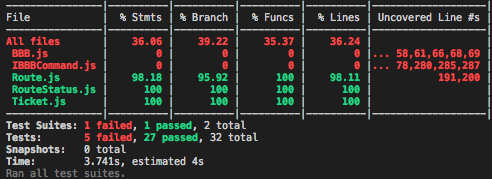
\includegraphics[width=.9\linewidth]{./Iteration2.rtfd/Pasted Graphic 1.tiff.png}
\end{center}

\subsubsection{Identify Missing Tests}
\label{sec:org50f68f1}

\begin{center}
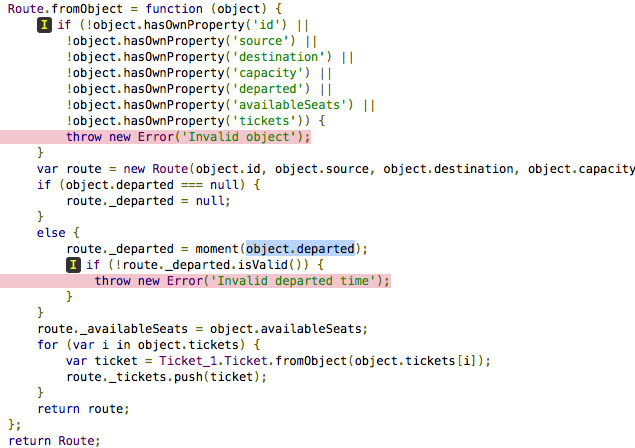
\includegraphics[width=.9\linewidth]{./Iteration2.rtfd/1_Pasted Graphic 2.tiff.png}
\end{center}



\begin{description}
\item[{TC\_Route\_26}] fromObject fails on invalid object
\begin{description}
\item[{Class}] Route
\item[{Method}] fromObject
\item[{Precondition}] N/A
\item[{Input}] \{ id\_X: “R1”, source: “Madrid”, destination: “Toledo”, capacity: 10,  tickets: [], departed: null, availableSeats: [0, 1, 2, 3, 4, 5, 6, 7, 8, 9]\}
\item[{Expected Output}] Error(‘Invalid object’)
\item[{Note}] The date set for departed is an example
\end{description}

\item[{TC\_Route\_27}] fromObject fails on invalid departure time
\begin{description}
\item[{Class}] Route
\item[{Method}] fromObject
\item[{Precondition}] N/A
\item[{Input}] \{ id: “R1”, source: “Madrid”, destination: “Toledo”, capacity: 10,  tickets: [], departed: “4711”, availableSeats: [0, 1, 2, 3, 4, 5, 6, 7, 8, 9]\}
\item[{Expected Output}] Error(‘Invalid departed time’)
\end{description}
\end{description}


Detected new failure in TC\_Route\_27
Pasted Graphic 6.tiff ¬


TC\_Route\_27:    fromObject fails on invalid departure time
Input:      \{ id: “R1”, source: “Madrid”, destination: “Toledo”, capacity: 10,  tickets: [], departed: “4711”, availableSeats: [0, 1, 2, 3, 4, 5, 6, 7, 8, 9]\}
Expected Output:  Error(‘Invalid departed time’)
Observed Output:  \{ id: “R1”, source: “Madrid”, destination: “Toledo”, capacity: 10,  tickets: [], departed: “4711-01-01T00:00:00.000Z”, availableSeats: [0, 1, 2, 3, 4, 5, 6, 7, 8, 9]\}


Pasted Graphic 8.tiff ¬

Fault: moment is not parsed enforcing ISO\_8601 date format

Fix: parse enforcing ISO\_8601 date format
Pasted Graphic 7.tiff ¬


Passing all tests and 100\% coverage
Pasted Graphic 9.tiff ¬

\subsection{Trace failures to faults}
\label{sec:orgcd6eeb9}

\subsubsection{TC\_Route\_6, TC\_Route\_7, TC\_Route\_8, TC\_Route\_9}
\label{sec:orgfc454a6}

\begin{description}
\item[{Failure}] Output is a number instead of a readable message.
\item[{Fault}] Method \texttt{status()} returns \texttt{enum} value instead of \texttt{string}:
\begin{center}
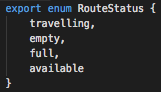
\includegraphics[width=.9\linewidth]{./Iteration2.rtfd/Pasted Graphic 4.tiff.png}
\end{center}
\item[{Fix}] Assign values to \texttt{enum}:
\begin{center}
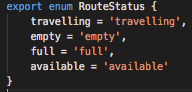
\includegraphics[width=.9\linewidth]{./Iteration2.rtfd/Pasted Graphic 5.tiff.png}
\end{center}
\end{description}

\subsubsection{TC\_Route\_15}
\label{sec:orgdc64618}

\begin{description}
\item[{Failure}] Number of available seats is not increased on a
cancellation.
\item[{Fault}] \texttt{cancelTicket} does remove the Ticket from the list of Tickets but
does not add the seat of the ticket back to the list of available
seats:
\begin{center}
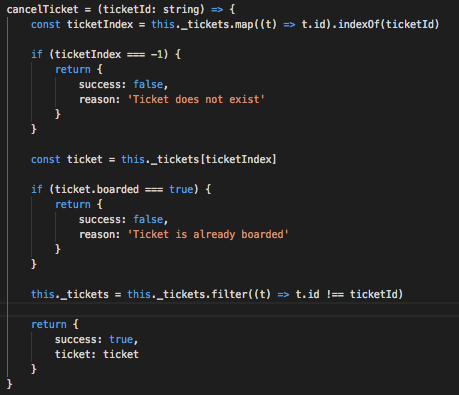
\includegraphics[width=.9\linewidth]{./Iteration2.rtfd/Pasted Graphic 2.tiff.png}
\end{center}
\item[{Fix}] Added the seat of the ticket to the list of available seats:
\begin{center}
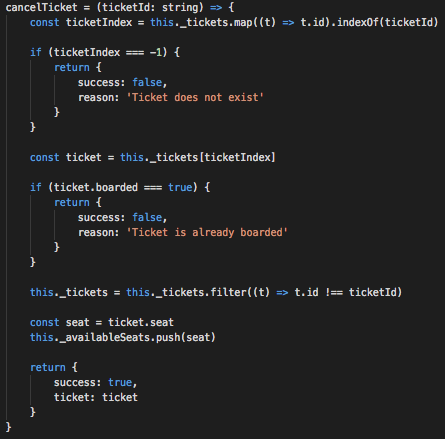
\includegraphics[width=.9\linewidth]{./Iteration2.rtfd/1_Pasted Graphic 3.tiff.png}
\end{center}
\end{description}

\subsubsection{TC\_RegisterRouteCommand\_4}
\label{sec:orgea09dde}

\begin{description}
\item[{Failure}] \texttt{TypeError} instead of error message
\item[{Fault}] \texttt{args[1]} is \texttt{null} and \texttt{trim()} cannot be called on \texttt{null}
\begin{center}
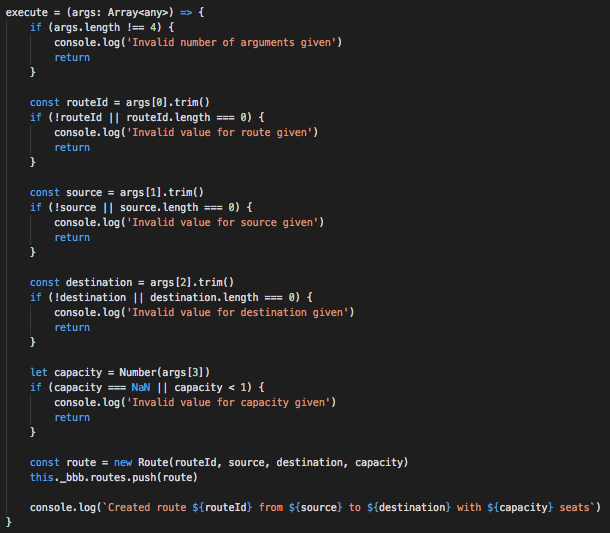
\includegraphics[width=.9\linewidth]{./Iteration3.rtfd/Pasted Graphic 7.tiff.png}
\end{center}
\item[{Fix}] Check that \texttt{args[1]} is not \texttt{null}
\begin{center}
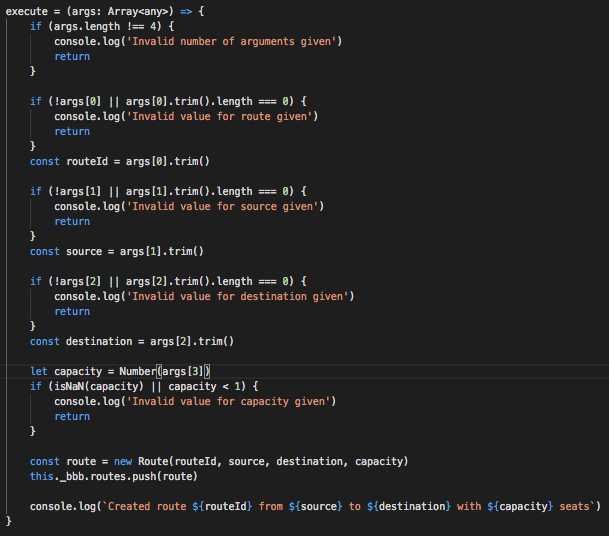
\includegraphics[width=.9\linewidth]{./Iteration3.rtfd/Pasted Graphic 14.tiff.png}
\end{center}
\end{description}

\subsubsection{TC\_RegisterRouteCommand\_5}
\label{sec:orgee0da37}

Same as with TC\_RegisterRouteCommand\_4 but with \texttt{args[2]}

\subsubsection{TC\_RegisterRouteCommand\_6}
\label{sec:orgd54438d}

\begin{description}
\item[{Failure}] \texttt{RangeError} instead of Error message
\item[{Fault}] Using \texttt{=== NaN} always yields false
\item[{Fix}] Use of \texttt{isNaN}
\end{description}

\subsubsection{TC\_DepartCommand\_3}
\label{sec:org705fb0a}

Test case was poorly specified (the observed output is correct and the
expected one is not):
\begin{itemize}
\item Title: fails for not existing Route
\item Expected Output: Console(“Route R\_X does not exist”)
\end{itemize}


\begin{description}
\item[{Fix}] Test case adapted
\end{description}

\subsubsection{TC\_BuyCommand\_3}
\label{sec:org94b186d}

\begin{description}
\item[{Failure}] \texttt{TypeError} instead of just error message
\item[{Fault}] Missing \texttt{return} statement after error message
\begin{center}
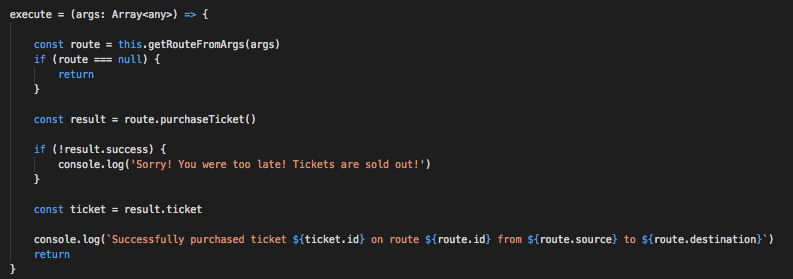
\includegraphics[width=.9\linewidth]{./Iteration3.rtfd/Pasted Graphic 9.tiff.png}
\end{center}
\item[{Fix}] \texttt{return} statement added
\begin{center}
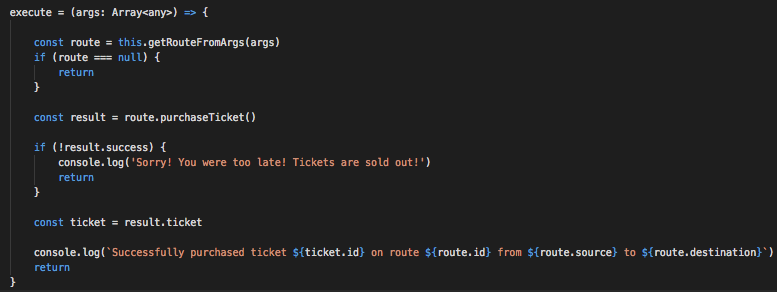
\includegraphics[width=.9\linewidth]{./Iteration3.rtfd/Pasted Graphic 16.tiff.png}
\end{center}
\end{description}

\subsubsection{TC\_CheckinCommand\_2}
\label{sec:org5044a19}

\begin{description}
\item[{Failure}] Additional wrong error message printed
\item[{Fault}] Missing \texttt{null} check for \texttt{ticketId}
\begin{center}
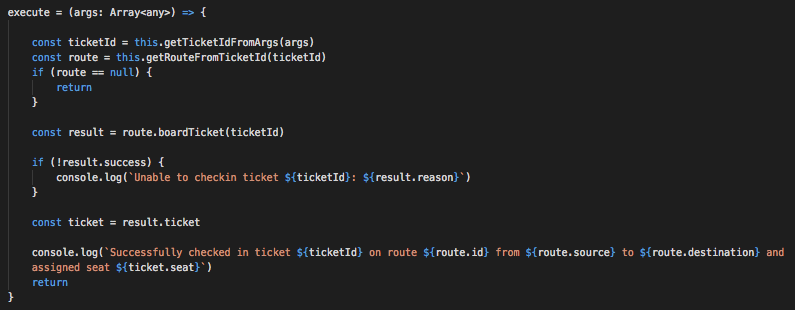
\includegraphics[width=.9\linewidth]{./Iteration3.rtfd/Pasted Graphic 10.tiff.png}
\end{center}
\item[{Fix}] Added \texttt{null} check for \texttt{ticketId}
\end{description}

\subsubsection{TC\_CheckinCommand\_3}
\label{sec:org7c13df2}

Same as TC\_CheckinCommand\_2

\subsubsection{TC\_CheckinCommand\_5}
\label{sec:orgbf3b162}

\begin{description}
\item[{Failure}] \texttt{TypeError} instead of just error message
\item[{Fault}] Missing return after error message
\begin{center}
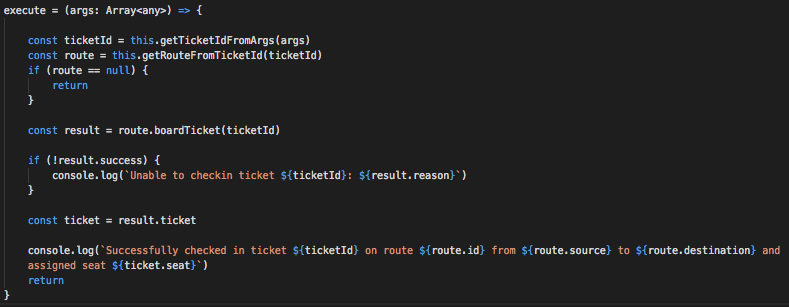
\includegraphics[width=.9\linewidth]{./Iteration3.rtfd/Pasted Graphic 11.tiff.png}
\end{center}
\item[{Fix}] Added \texttt{return} statement
\end{description}

\subsubsection{TC\_CancelCommand\_2}
\label{sec:orgec90d75}

\begin{description}
\item[{Failure}] Additional wrong error message printed
\item[{Fault}] Missing \texttt{null} check for \texttt{ticketId}
\begin{center}
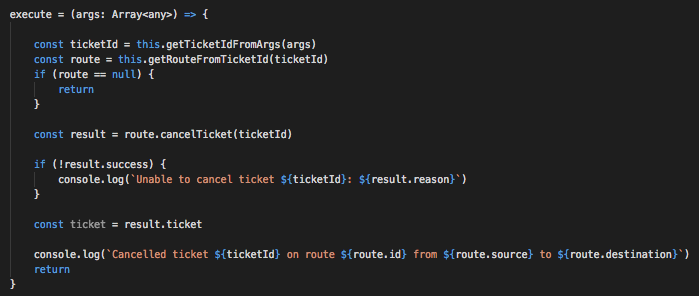
\includegraphics[width=.9\linewidth]{./Iteration3.rtfd/Pasted Graphic 12.tiff.png}
\end{center}
\item[{Fix}] Added \texttt{null} check for \texttt{ticketId}
\end{description}

\subsubsection{TC\_CancelCommand\_3}
\label{sec:org6e20a8b}

Same as TC\_CancelCommand\_2

\subsubsection{TC\_CancelCommand\_5}
\label{sec:orga548309}

\begin{description}
\item[{Failure}] Wrong message printed, ticket data falsely manipulated
\item[{Fault}] Missing return after error message
\begin{center}
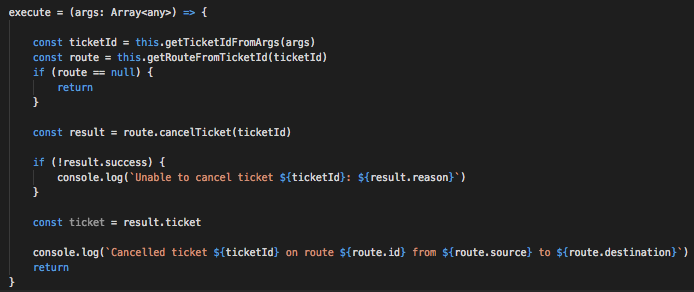
\includegraphics[width=.9\linewidth]{./Iteration3.rtfd/Pasted Graphic 13.tiff.png}
\end{center}
\item[{Fix}] Added \texttt{return} statement
\end{description}
\end{document}
